\documentclass[border=4pt,12pt]{standalone}
% House style for redrawn exam diagrams (diagram-v4: 0.4pt lines, filled -latex arrows, fine dashes; stipple and hatching drawn as real dots/lines (no PDF/SVG patterns, so they render in every browser and at any scale); transparent background). Every figure \input's this.
\usepackage{amsmath,amssymb}
\usepackage{txfonts}
\usepackage{pdfrender,xcolor}
% \halo{text}: label on shading. The shading stops just around each letter's outline (a thin knock-out that follows the
% glyphs, like the papers' typesetting), never a box. Owner: "I don't want a box around the text".
\newcommand{\halo}[1]{\leavevmode\rlap{\pdfrender{TextRenderingMode=2,LineWidth=2.2pt,LineJoinStyle=1,StrokeColor=white,FillColor=white}#1}#1}
\usepackage{tikz,pgfplots}
\pgfplotsset{compat=1.18}
\usetikzlibrary{arrows.meta,calc,angles,quotes,patterns,patterns.meta,intersections,positioning,decorations.markings,shapes.geometric}
% Stipple and hatching are drawn as actual dots / lines clipped to the region (path picture), NOT as pattern fills:
% SVG <pattern> fills vanish or blur when browsers scale the image, so the owner could not see the shading.
% Each dot is a 0.72pt square (keeps SVGs small; reads as a dot at print size). Dots sit on one global staggered grid, so neighbouring regions line up.
\makeatletter
\newdimen\ex@x \newdimen\ex@y \newdimen\ex@xa \newdimen\ex@ya \newdimen\ex@xb \newdimen\ex@yb \newcount\ex@row
\def\exam@stipplecolor{black!75}\def\exam@dotr{0.42pt}\def\exam@dotgap{2.5}
\def\ex@rowdots{\ifdim\ex@x<\ex@xb \pgfpathrectangle{\pgfqpoint{\dimexpr\ex@x-0.36pt\relax}{\dimexpr\ex@y-0.36pt\relax}}{\pgfqpoint{0.72pt}{0.72pt}}\advance\ex@x by \exam@dotgap pt\relax\expandafter\ex@rowdots\fi}
\def\exam@stipple{%
  \pgftransformreset% dots are sized in real points even inside scaled pictures
  \pgfpointanchor{path picture bounding box}{south west}\ex@xa=\pgf@x \ex@ya=\pgf@y
  \pgfpointanchor{path picture bounding box}{north east}\ex@xb=\pgf@x \ex@yb=\pgf@y
  \pgfsetfillcolor{\exam@stipplecolor}\pgfmathsetmacro\ex@h{\exam@dotgap/2}%
  \pgfmathtruncatemacro\ex@r{floor(\ex@ya/\ex@h)-1}\ex@row=\ex@r\relax
  \ex@y=\ex@r\dimexpr\ex@h pt\relax
  \loop\ifdim\ex@y<\ex@yb
    \pgfmathtruncatemacro\ex@c{floor(\ex@xa/\exam@dotgap)-1}\ex@x=\ex@c\dimexpr\exam@dotgap pt\relax
    \ifodd\ex@row \advance\ex@x by \ex@h pt\fi
    \ex@rowdots
    \advance\ex@y by \ex@h pt \advance\ex@row by 1
    \ifnum\numexpr\ex@row-(\ex@row/4)*4\relax=0 \pgfusepath{fill}\fi% flush every 4 rows: bounded TeX memory, few clip copies in the SVG
  \repeat\pgfusepath{fill}}
\newdimen\ex@d
\def\exam@hatch#1{% #1 = 1 for /, -1 for \ ; lines 45 degrees, 3pt apart
  \pgftransformreset
  \pgfpointanchor{path picture bounding box}{south west}\ex@xa=\pgf@x \ex@ya=\pgf@y
  \pgfpointanchor{path picture bounding box}{north east}\ex@xb=\pgf@x \ex@yb=\pgf@y
  \ex@d=\dimexpr\ex@yb-\ex@ya\relax \ex@x=\dimexpr\ex@xa-\ex@d\relax
  \loop\ifdim\ex@x<\ex@xb
    \ifnum#1>0 \pgfpathmoveto{\pgfqpoint{\ex@x}{\ex@ya}}\pgfpathlineto{\pgfqpoint{\dimexpr\ex@x+\ex@d\relax}{\ex@yb}}%
    \else \pgfpathmoveto{\pgfqpoint{\ex@x}{\ex@yb}}\pgfpathlineto{\pgfqpoint{\dimexpr\ex@x+\ex@d\relax}{\ex@ya}}\fi
    \advance\ex@x by 4.24pt
  \repeat
  \pgfsetlinewidth{0.4pt}\pgfsetstrokecolor{black}\pgfusepath{stroke}}
\def\examstipple{\exam@stipple}\def\examhatch{\exam@hatch}\def\examsetstipplecolor#1{\def\exam@stipplecolor{#1}}\def\examsetdotgap#1{\def\exam@dotgap{#1}}
\makeatother
% (legacy pattern kept for old files)
% staggered stipple like the NESA papers' dotted shading
\pgfdeclarepatternformonly{exam stipple}{\pgfpointorigin}{\pgfqpoint{2.2pt}{2.2pt}}{\pgfqpoint{2.2pt}{2.2pt}}{%
  \pgfpathcircle{\pgfqpoint{0.55pt}{0.55pt}}{0.42pt}\pgfpathcircle{\pgfqpoint{1.65pt}{1.65pt}}{0.42pt}\pgfusepath{fill}}
\tikzset{
  every picture/.style={line width=0.6pt, >={Latex[length=2mm,width=1.3mm]}},
  curve/.style={line width=0.6pt},
  open arrow/.style={-{Latex[length=2mm,width=1.3mm]}},  % owner: filled -latex heads everywhere, no open chevrons
  aux/.style={dash pattern=on 2pt off 1.5pt, line width=0.6pt},
  shade/.code={\def\exA{#1}\def\exB{none}\ifx\exA\exB\else\pgfkeysalso{fill=black!18}\fi},
  shade/.default=on,
  shade dots/.style={fill=none, path picture={\examstipple}},
  stipple color/.code={\examsetstipplecolor{#1}},
  stipple gap/.code={\examsetdotgap{#1}},
  shade dense dots/.style={fill=none, stipple gap=1.6, path picture={\examstipple}},
  shade hatch/.style={fill=none, path picture={\examhatch{1}}},
  shade hatch reverse/.style={fill=none, path picture={\examhatch{-1}}},
  shade solid/.style={fill=black},
  pt/.style={circle, fill, inner sep=1.1pt},
  open pt/.style={circle, draw, fill=white, inner sep=1.1pt},
}
\pgfplotsset{
  exam axes/.style={axis lines=middle, axis line style={->}, xlabel={$x$}, ylabel={$y$},
    xlabel style={anchor=west}, ylabel style={anchor=south}, tick label style={font=\small},
    every axis plot/.append style={line width=0.6pt, black}, samples=200, clip=false,
    enlargelimits=false, axis on top},
}

\begin{document}
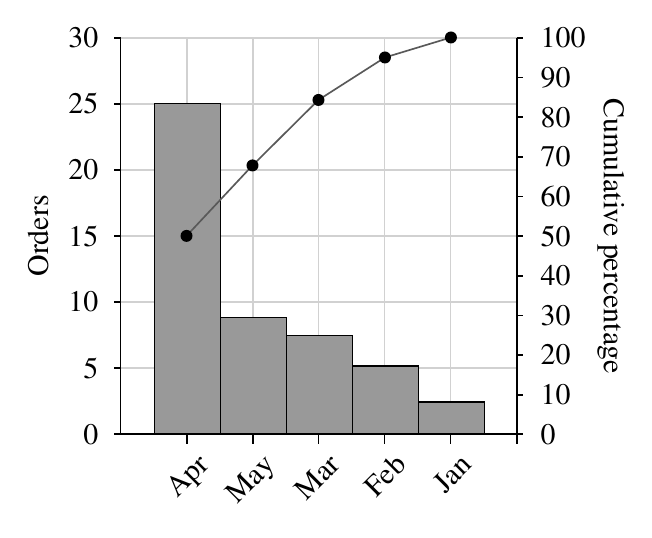
\begin{tikzpicture}[x=0.0127cm,y=-0.0127cm,every node/.style={font=\fontsize{10.8}{12.96}\selectfont}]
\draw[black!18] (182,23) -- (182,419.5);
\draw[black!18] (248,23) -- (248,419.5);
\draw[black!18] (313.5,23) -- (313.5,419.5);
\draw[black!18] (379.5,23) -- (379.5,419.5);
\draw[black!18] (445.5,23) -- (445.5,419.5);
\draw[black!18] (115.5,23) -- (512,23);
\draw[black!18] (115.5,89) -- (512,89);
\draw[black!18] (115.5,155) -- (512,155);
\draw[black!18] (115.5,221) -- (512,221);
\draw[black!18] (115.5,287) -- (512,287);
\draw[black!18] (115.5,353) -- (512,353);
\draw[fill=black!40] (149.5,419.5) rectangle (215.5,88.5);
\draw[fill=black!40] (215.5,419.5) rectangle (281.5,302.5);
\draw[fill=black!40] (281.5,419.5) rectangle (347.5,320.5);
\draw[fill=black!40] (347.5,419.5) rectangle (413.5,351);
\draw[fill=black!40] (413.5,419.5) rectangle (479.5,387);
\draw (115.5,23) -- (115.5,419.5) -- (512,419.5) -- (512,23);
\draw (109,419.5) -- (115.5,419.5); \node[anchor=east,inner sep=0] at (94,419.5) {0};
\draw (109,353.4) -- (115.5,353.4); \node[anchor=east,inner sep=0] at (94,353.4) {5};
\draw (109,287.3) -- (115.5,287.3); \node[anchor=east,inner sep=0] at (94,287.3) {10};
\draw (109,221.2) -- (115.5,221.2); \node[anchor=east,inner sep=0] at (94,221.2) {15};
\draw (109,155.1) -- (115.5,155.1); \node[anchor=east,inner sep=0] at (94,155.1) {20};
\draw (109,89.0) -- (115.5,89.0); \node[anchor=east,inner sep=0] at (94,89.0) {25};
\draw (109,22.9) -- (115.5,22.9); \node[anchor=east,inner sep=0] at (94,22.9) {30};
\draw (512,419.5) -- (518.5,419.5); \node[anchor=west,inner sep=0] at (535,419.5) {0};
\draw (512,379.9) -- (518.5,379.9); \node[anchor=west,inner sep=0] at (535,379.9) {10};
\draw (512,340.2) -- (518.5,340.2); \node[anchor=west,inner sep=0] at (535,340.2) {20};
\draw (512,300.6) -- (518.5,300.6); \node[anchor=west,inner sep=0] at (535,300.6) {30};
\draw (512,260.9) -- (518.5,260.9); \node[anchor=west,inner sep=0] at (535,260.9) {40};
\draw (512,221.2) -- (518.5,221.2); \node[anchor=west,inner sep=0] at (535,221.2) {50};
\draw (512,181.6) -- (518.5,181.6); \node[anchor=west,inner sep=0] at (535,181.6) {60};
\draw (512,141.9) -- (518.5,141.9); \node[anchor=west,inner sep=0] at (535,141.9) {70};
\draw (512,102.3) -- (518.5,102.3); \node[anchor=west,inner sep=0] at (535,102.3) {80};
\draw (512,62.7) -- (518.5,62.7); \node[anchor=west,inner sep=0] at (535,62.7) {90};
\draw (512,23.0) -- (518.5,23.0); \node[anchor=west,inner sep=0] at (535,23.0) {100};
\draw (182,419.5) -- (182,429);
\draw (248,419.5) -- (248,429);
\draw (313.5,419.5) -- (313.5,429);
\draw (379.5,419.5) -- (379.5,429);
\draw (445.5,419.5) -- (445.5,429);
\draw (512,419.5) -- (512,429);
\draw[black!65] (181.5,221) -- (247.5,150.5) -- (313.5,85) -- (380,42.5) -- (446,22.5);
\fill (181.5,221) circle (6);
\fill (247.5,150.5) circle (6);
\fill (313.5,85) circle (6);
\fill (380,42.5) circle (6);
\fill (446,22.5) circle (6);
\node[rotate=45,anchor=north east,inner sep=0] at (191,436) {Apr};
\node[rotate=45,anchor=north east,inner sep=0] at (257,436) {May};
\node[rotate=45,anchor=north east,inner sep=0] at (322.5,436) {Mar};
\node[rotate=45,anchor=north east,inner sep=0] at (388.5,436) {Feb};
\node[rotate=45,anchor=north east,inner sep=0] at (454.5,436) {Jan};
\node[rotate=90,inner sep=0] at (33,221) {Orders};
\node[rotate=-90,inner sep=0] at (606,221) {Cumulative percentage};
\end{tikzpicture}
\end{document}
